
\documentclass[10pt]{beamer}
\usetheme{metropolis}

% ── Packages ──
\usepackage{amsmath,amssymb,amsthm}
\usepackage{tikz}
\usetikzlibrary{positioning,arrows.meta,fit,matrix,backgrounds,calc,shapes.geometric,decorations.pathreplacing}
\usepackage{graphicx}
\usepackage{array}
\usepackage{etoolbox}
\usepackage{cancel}

% ── Theorem environments ──
\theoremstyle{definition}
\newtheorem{defi}{Definition}[section]
\newtheorem{prop}{Proposition}[section]
\newtheorem{thm}{Theorem}[section]
\newtheorem{cor}{Corollary}[section]

% Custom theorem styles with colors
\setbeamercolor{block title}{bg=red!75!black,fg=white}
\setbeamercolor{block body}{bg=yellow!10!white}

\AtBeginEnvironment{prop}{%
  \setbeamercolor{block title}{bg=yellow!75!black,fg=black}%
  \setbeamercolor{block body}{bg=yellow!10!white}%
}
\AtEndEnvironment{prop}{%
  \setbeamercolor{block title}{bg=red!75!black,fg=white}%
}

\AtBeginEnvironment{thm}{%
  \setbeamercolor{block title}{bg=yellow!75!black,fg=black}%
  \setbeamercolor{block body}{bg=yellow!10!white}%
}
\AtEndEnvironment{thm}{%
  \setbeamercolor{block title}{bg=red!75!black,fg=white}%
}

\AtBeginEnvironment{cor}{%
  \setbeamercolor{block title}{bg=yellow!75!black,fg=black}%
  \setbeamercolor{block body}{bg=yellow!10!white}%
}
\AtEndEnvironment{cor}{%
  \setbeamercolor{block title}{bg=red!75!black,fg=white}%
}

% ── Highlighting ──
\newcommand{\x}[1]{\alert{\textbf{#1}}}

% ── Color shortcuts ──
\newcommand{\rd}[1]{{\color{red!70!black}#1}}
\newcommand{\bl}[1]{{\color{blue!70!black}#1}}
\newcommand{\gn}[1]{{\color{green!60!black}#1}}

\title{Lecture 15: Spectral Decomposition}
\subtitle{MATH203 Applied Linear Algebra}
\date{}
\titlegraphic{}

\begin{document}
\maketitle


% ┌─────────────────────────────────────────────────────────────────────┐
% │ SECTION-LEVEL ADR: THE HOOK — WHY DOES $A^n$ MATTER?              │
% │                                                                    │
% │ THE MACRO DESIGN: PROBLEM-FIRST RAPPORT                           │
% │                                                                    │
% │ The audience enters this lecture knowing Cayley-Hamilton from L14. │
% │ They can reduce A^2 to 5A+2I. But they don't yet feel the PAIN   │
% │ of not having a closed formula. This section manufactures that     │
% │ pain by posing three real problems — recurrence, probability,      │
% │ money sharing — all of which REDUCE to A^n but CANNOT be solved   │
% │ efficiently with L14's step-by-step method.                        │
% │                                                                    │
% │ Phase 1 — HOOK (Frame 1): Open with a PROBLEM, not a topic.       │
% │   "What is a_{100}?" — the audience immediately has a task.        │
% │   This is the same "start with shared experience" technique from   │
% │   L07's sunlight model, except here the shared experience is the   │
% │   frustration of a sequence they can't easily compute.             │
% │                                                                    │
% │ Phase 2 — AMPLIFY (Frames 2-3): Two more problems, same shape.    │
% │   The audience realizes: this isn't one problem, it's a whole      │
% │   CLASS of problems. The weight of three unsolved problems         │
% │   creates genuine need for a solution.                             │
% │                                                                    │
% │ Phase 3 — FRUSTRATE (Frame 4): L14's method fails at scale.       │
% │   Show A^3, A^4, A^5 step by step. Each requires its own calc.    │
% │   Want A^{100}? Repeat 99 times. The audience FEELS the           │
% │   inadequacy of the old tool. This is manufactured frustration     │
% │   — but honest frustration, because the limitation is real.        │
% │                                                                    │
% │ Phase 4 — WHITESPACE + DREAM (Frames 5-6): Scene change.          │
% │   The whitespace frame asks the question the audience is already   │
% │   thinking: "Is there a closed formula?" Then the projection       │
% │   dream answers it: if A is a sum of projections, A^n is instant.  │
% │   The gap between "I need this" and "here it is" fires the same   │
% │   micro-dopamine hit described in L07's narrative engine ADR.      │
% │                                                                    │
% │ NARRATIVE ENGINE: TENSION → REVEAL → JUSTIFY                      │
% │   TENSION: three unsolved problems + L14's painful method          │
% │   REVEAL: projections make A^n trivial (Frame 6)                   │
% │   JUSTIFY: will come in §3-4 when Lagrange delivers the proof     │
% │                                                                    │
% │ WHY THREE PROBLEMS (not one):                                      │
% │   One problem is an exercise. Three problems from different        │
% │   domains (sequences, probability, economics) make A^n feel        │
% │   UNIVERSAL — "this matters everywhere, not just in one homework   │
% │   problem." The weight justifies the machinery we're about to      │
% │   build. A student who sees one recurrence might think "niche."    │
% │   A student who sees recurrence + probability + money thinks       │
% │   "I need this for my career."                                     │
% │                                                                    │
% │ WHY NOT START WITH EIGENVALUE DEFINITION:                          │
% │   Textbooks open with "Definition: λ is an eigenvalue if..."       │
% │   This is efficient but alienating. The student has no reason to   │
% │   care. Our opening manufactures the NEED before the tool.         │
% └─────────────────────────────────────────────────────────────────────┘
\section{Why Do We Need $A^n$?}


% ADR: Open with a PROBLEM, not a topic. The audience reads a_{100} and
% immediately wants to know the answer. The recurrence is simple enough
% that anyone can compute a_0=0, a_1=1, a_2=3, a_3=7, a_4=15... but the
% pattern (2^n - 1) is not obvious from the numbers alone.
% AUDIENCE EMOTION: curiosity — "what IS a_{100}?" (hooked by a concrete question)
% AUDIENCE ATTENTION: active — they're computing the first few terms in their heads
\begin{frame}{What Is $a_{100}$?}

$$a_0 = 0, \qquad a_1 = 1, \qquad a_{n+1} = 3a_n - 2a_{n-1}$$

\vfill\pause

The first few terms: $\quad 0, \; 1, \; 3, \; 7, \; 15, \; 31, \; \ldots$

\vfill\pause

Rewrite as a matrix recurrence:
$$\begin{pmatrix}a_{n+1}\\a_n\end{pmatrix} = \underbrace{\begin{pmatrix}3&-2\\1&0\end{pmatrix}}_{B}\begin{pmatrix}a_n\\a_{n-1}\end{pmatrix}$$

\vfill

After $n$ steps:
$$\begin{pmatrix}a_{n+1}\\a_n\end{pmatrix} = B^n\begin{pmatrix}1\\0\end{pmatrix}$$

\vfill

To answer the question, we need $B^{100}$.

\end{frame}


% ADR: Two more problems from DIFFERENT worlds — probability and economics.
% The audience sees: this isn't one isolated problem, it's a universal pattern.
% Each problem is stated AS A PROBLEM (question mark!), not as an observation.
% AUDIENCE EMOTION: growing weight — "ok, A^n comes up EVERYWHERE"
% AUDIENCE ATTENTION: the variety (coins, money) keeps them engaged;
% the repetition (→ matrix → A^n) hammers the pattern.
\begin{frame}[shrink=5]{$A^n$ Is Everywhere}

\textbf{Probability.}\; Flip a coin repeatedly.
Heads $\to$ walk \x{3} meters. \; Tails $\to$ walk \x{2} meters.

What is the probability of landing \x{exactly} on the $n$-meter mark?

\vfill

$$p_n = \tfrac{1}{2}\,p_{n-2} + \tfrac{1}{2}\,p_{n-3} \qquad\longrightarrow\qquad \text{need } A^n$$

\vfill\pause

\textbf{Money sharing.}\; Three cousins each start with some money.

Each round: pool half your money, split the pool equally.

\vfill

$$\vec{m}_n = \underbrace{\begin{pmatrix}2/3&1/6&1/6\\1/6&2/3&1/6\\1/6&1/6&2/3\end{pmatrix}}_{M} \vec{m}_{n-1}
\qquad\longrightarrow\qquad \text{need } M^n$$

\vfill

What happens as $n \to \infty$? \; Does everyone end up with the same amount?

\end{frame}


% ADR: FRUSTRATE — show that L14's method breaks at scale.
% The audience sees: A^3 requires A^2. A^4 requires A^3. Each step is
% its own computation. Want A^{100}? Do it 99 times.
% The numbers get ugly fast (145, 781) — this is by design.
% AUDIENCE EMOTION: frustration — "there MUST be a better way"
% AUDIENCE ATTENTION: the growing numbers are visually overwhelming,
% which is the point. The vdots + "repeat 99 times" is the kill shot.
%
% WHY SHOW THE UGLY NUMBERS: If we just SAID "it's painful," the audience
% wouldn't feel it. By writing out 145A + 54I, 781A + 290I, we make the
% pain visceral. The growing coefficients are evidence, not decoration.
\begin{frame}{Lecture 14's Method: One Step at a Time}

Lecture 14 taught us: $A^2 = 5A + 2I$ for $A = \begin{pmatrix}1&2\\3&4\end{pmatrix}$.

\vfill

\begin{align*}
A^3 &= A \cdot A^2 = A(5A + 2I) = 5A^2 + 2A = 27A + 10I \\
A^4 &= A \cdot A^3 = 145A + 54I \\
A^5 &= 781A + 290I \\
     &\;\;\vdots
\end{align*}

\vfill\pause

Each power needs \x{the previous power}.

\vfill

Want $A^{100}$? \quad Repeat \x{99 times}.

\vfill

This is not a formula. This is bookkeeping.

\end{frame}


% ADR: WHITESPACE TRANSITION — the scene change.
% Empty space + big question signals: we are leaving the problem world
% and entering the solution world. The audience has been frustrated for
% three slides; the whitespace lets the frustration crystallize into a
% question they actively WANT answered.
% AUDIENCE EMOTION: anticipation — "please tell me there's a better way"
% AUDIENCE ATTENTION: whitespace resets attention (L07 ADR principle)
\begin{frame}{}

\vfill

\begin{center}
{\Large Can we find a \x{closed formula} for $A^n$?}

\vspace{1cm}

{\large Just plug in $n$ --- get the answer immediately?}
\end{center}

\vfill

\end{frame}


% ADR: THE REVEAL — projections are the key.
% This is the answer to the whitespace question. We don't explain WHY
% it works yet (that's §3-4). We just show the DREAM: if A = 2P_1 + 3P_2,
% then A^n = 2^n P_1 + 3^n P_2. The audience holds the answer and
% WANTS to verify it — they are pulled toward the abstraction.
%
% NARRATIVE ENGINE position: this is the REVEAL at peak tension.
% The justification comes later (Lagrange in §3, Cayley-Hamilton in §4).
%
% The slogan box at the bottom is the "bumper sticker" — something
% students remember even if they forget the details.
% AUDIENCE EMOTION: hope — "this could actually work!"
% AUDIENCE ATTENTION: the boxed formula A^n = 2^n P_1 + 3^n P_2 is
% visually striking; the underbrace "= P_1" makes P^n = P visceral.
\begin{frame}[shrink=2]{The Goal: What Would the Ideal Formula Look Like?}

We don't know the answer yet. But let's \x{imagine} the best possible outcome.

\vfill

From Lectures 7--10, you know \x{projections}:
$$P^2 = P \;\implies\; P^n = P \quad\text{for all } n \geq 1.$$

\vfill\pause

\x{If} we could somehow write $A = 2 P_1 + 3 P_2$ for projections $P_1, P_2$, then:

$$A^n = 2^n\!\cdot\!\underbrace{P_1^n}_{= P_1} + 3^n\!\cdot\!\underbrace{P_2^n}_{= P_2} = \boxed{2^n P_1 + 3^n P_2}$$

\vfill\pause

A \x{closed formula}. Plug in $n = 100$? Done.

\vfill

This is \x{the formula we want to arrive at} by the end of this lecture.

\vfill

\begin{center}
\fbox{\parbox{0.8\textwidth}{\centering
\x{Slogan}: Projections are the simplest matrices.\\[3pt]
To understand any matrix, decompose it into projections.
}}
\end{center}

\end{frame}


% ┌─────────────────────────────────────────────────────────────────────┐
% │ SECTION-LEVEL ADR: NAMING THE INGREDIENTS                          │
% │                                                                    │
% │ The audience now has a dream: decompose A into weighted             │
% │ projections. Before we can BUILD the decomposition (§3-4), we      │
% │ need to NAME the ingredients: eigenvalues and eigenvectors.        │
% │                                                                    │
% │ This section is the TRANSLATION phase (cf. L07 Phase 2): we       │
% │ take the visual intuition ("some vectors just get scaled") and     │
% │ give it precise mathematical language.                             │
% │                                                                    │
% │ WHY NOT DEFINE FIRST AND MOTIVATE LATER:                           │
% │ Textbooks say "Definition: eigenvalue..." then ask "why care?"     │
% │ We reversed it: the audience already CARES (they need A^n), so    │
% │ the definition feels like naming something they already want.      │
% │                                                                    │
% │ The geometric TikZ picture comes BEFORE the definition — concrete  │
% │ before abstract. The student sees the behavior, then gets the word │
% │ for it. "Oh, THAT'S what an eigenvector is."                       │
% │                                                                    │
% │ The section ends with a WHITESPACE QUESTION: "How do we find the  │
% │ projections?" This launches §3.                                    │
% └─────────────────────────────────────────────────────────────────────┘
\section{Eigenvalues and Eigenvectors}


% ADR: BRIDGE FRAME — transition from algebraic (§1) to geometric (§2).
% §1 was entirely algebraic: A^n, recurrences, the dream formula.
% §2 opens with a geometric picture (vectors getting scaled).
% Without a bridge, the audience feels a jarring jump. This frame
% says: "we've seen the algebraic goal; now let's look at what happens
% GEOMETRICALLY when A acts on vectors."
% AUDIENCE EMOTION: orientation — "oh, we're changing perspective now"
% AUDIENCE ATTENTION: whitespace resets; the question refocuses them.
\begin{frame}{}

\vfill

\begin{center}
{\Large We've seen the \x{algebraic} goal:}

\vspace{0.5cm}

{\large decompose $A$ into a sum of projections.}

\vspace{1cm}

{\Large Now: what happens \x{geometrically}?}

\vspace{0.5cm}

{\large When $A$ acts on a vector, which vectors ``survive''?}
\end{center}

\vfill

\end{frame}


% ADR: Geometry BEFORE definition. The audience sees the picture first,
% then gets the vocabulary. The TikZ diagram uses three vectors:
%   - red eigenvector (1,0): scaled by 2, same direction → "easy"
%   - blue eigenvector (1,-1): unchanged → "trivially easy"
%   - gray non-eigenvector (1,1) → (3,1): direction changes → "hard"
% The visual contrast between "stays on the line" and "goes off the line"
% is the entire concept of eigenvector, before any formula.
%
% AUDIENCE EMOTION: visual understanding — "I SEE which vectors are special"
% AUDIENCE ATTENTION: three colored arrows create a natural comparison;
% the "direction changed!" label draws the eye to the contrast.
\begin{frame}[shrink=5]{Some Vectors Are Special}

Multiply three vectors by $M = \begin{pmatrix}2&1\\0&1\end{pmatrix}$:

\begin{center}
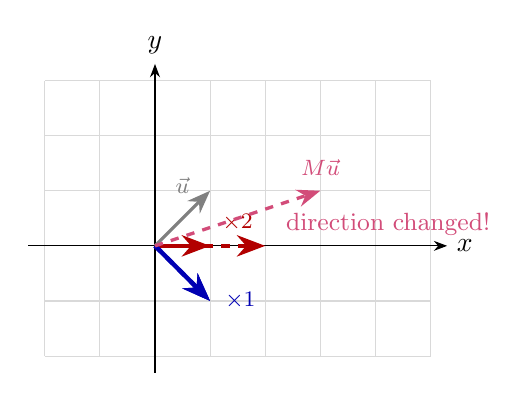
\begin{tikzpicture}[scale=0.7]
  \draw[gray!30, step=1] (-2,-2) grid (5,3);
  \draw[-{Stealth}] (-2.3,0) -- (5.3,0) node[right]{$x$};
  \draw[-{Stealth}] (0,-2.3) -- (0,3.3) node[above]{$y$};

  % Eigenvector: (1,0) -> (2,0), eigenvalue 2
  \draw[-{Stealth}, ultra thick, red!70!black] (0,0) -- (1,0);
  \draw[-{Stealth}, ultra thick, red!70!black, dashed] (0,0) -- (2,0);
  \node[red!70!black, above, font=\footnotesize] at (1.5,0.1) {$\times 2$};

  % Eigenvector: (1,-1) -> (1,-1), eigenvalue 1
  \draw[-{Stealth}, ultra thick, blue!70!black] (0,0) -- (1,-1);
  \draw[-{Stealth}, ultra thick, blue!70!black, dashed] (0,0) -- (1,-1);
  \node[blue!70!black, right, font=\footnotesize] at (1.1,-1) {$\times 1$};

  % Non-eigenvector: (1,1) -> (3,1), direction changes
  \draw[-{Stealth}, very thick, gray] (0,0) -- (1,1);
  \draw[-{Stealth}, very thick, purple!70, dashed] (0,0) -- (3,1);
  \node[gray, left, font=\footnotesize] at (0.8,1.1) {$\vec{u}$};
  \node[purple!70, above, font=\footnotesize] at (3,1.1) {$M\vec{u}$};
  \node[purple!70, right, font=\footnotesize] at (2.2,0.4) {\small direction changed!};
\end{tikzpicture}
\end{center}

\vfill

\rd{$\vec{v}_1 = (1,0)$}: stays on the same line, stretched by $2$.

\bl{$\vec{v}_2 = (1,-1)$}: stays on the same line, unchanged.

\vfill

These vectors just get \x{scaled}. No rotation, no shearing.

\end{frame}


% ADR: NOW name the phenomenon. The audience has seen the picture;
% the definition is just giving a name to something they already understand.
% The table of λ values gives physical meaning to each case.
% AUDIENCE EMOTION: "oh, THAT's what an eigenvector is" (naming relief)
% AUDIENCE ATTENTION: the table is scannable — each row is one scenario.
\begin{frame}{Definition: Eigenvalue and Eigenvector}

\begin{defi}
A \x{non-zero} vector $\vec{v}$ is an \x{eigenvector} of $A$ for \x{eigenvalue} $\lambda$ if
$$A\vec{v} = \lambda\vec{v}.$$
\end{defi}

\vfill

In words: $A$ acts on $\vec{v}$ by just \x{scaling}.

\vfill

\begin{center}
\renewcommand{\arraystretch}{1.4}
\begin{tabular}{cl}
$\lambda > 1$ & vector gets \x{stretched} \\
$0 < \lambda < 1$ & vector gets \x{shrunk} \\
$\lambda = 0$ & vector gets \x{killed} (sent to $\vec{0}$) \\
$\lambda < 0$ & vector gets \x{flipped} and scaled \\
$\lambda = 1$ & vector \x{doesn't move}
\end{tabular}
\end{center}

\end{frame}


% ADR: PROPOSITION — roots of det(tI-A) are eigenvalues.
% The definition said: eigenvalue = λ such that Av = λv for non-zero v.
% Now we PROVE that roots of det(tI-A) are eigenvalues. The proof uses
% two facts the students already know: (1) det = 0 ⟹ not full rank,
% (2) not full rank ⟹ non-trivial null space. This is a proposition,
% NOT a definition — the user explicitly flagged this logic gap.
%
% After the proof, introduce the RUNNING EXAMPLE that will carry
% through §3-4. Clean eigenvalues 0,1,2 for integer arithmetic.
% AUDIENCE EMOTION: "oh! the eigenvalues hide inside the determinant"
% AUDIENCE ATTENTION: the proof is short (3 lines) and uses familiar tools.
\begin{frame}[shrink=5]{Where Do Eigenvalues Come From?}

\begin{prop}
If $\lambda$ is a root of $\det(tI - A)$, then $\lambda$ is an \x{eigenvalue} of $A$.
\end{prop}

\vfill

\textbf{Proof.}\; $\lambda$ is a root means $\det(\lambda I - A) = 0$.

\medskip

$\det(\lambda I - A) = 0 \;\implies\;$ the matrix $(\lambda I - A)$ is \x{not invertible}.

\medskip

Not invertible $\implies$ the equation $(\lambda I - A)\vec{x} = \vec{0}$ has a \x{non-zero solution} $\vec{v}$.

\medskip

So $A\vec{v} = \lambda\vec{v}$ with $\vec{v} \neq \vec{0}$: that is exactly an eigenvector. \;\qed

\vfill\pause

\textbf{Running example for today}:

$$A = \begin{pmatrix}1&0&1\\0&1&0\\1&0&1\end{pmatrix}, \qquad \det(tI - A) = t(t-1)(t-2)$$

\vfill

Eigenvalues: $\lambda_1 = 0$, $\lambda_2 = 1$, $\lambda_3 = 2$.

\end{frame}


% ADR: THIS IS THE CRITICAL BRIDGE. The audience knows eigenvalues are
% roots of det(tI-A). Now we REMIND them what Cayley-Hamilton said:
% det(tI-A) is an ANNIHILATING polynomial — plug in t=A and you get 0.
% The factored form makes this concrete: (A-0I)(A-I)(A-2I) = 0.
%
% WHY THIS FRAME EXISTS: Without it, the audience has two disconnected
% facts: "eigenvalues are roots" (from §2) and "Lagrange divides by
% these roots" (in §3). The Cayley-Hamilton callback is the GLUE:
% it says WHY dividing by those factors matters — the product KILLS A.
%
% AUDIENCE EMOTION: "oh! the eigenvalues are exactly the factors in the
% annihilating polynomial!" (connection firing)
% AUDIENCE ATTENTION: the concrete equation A(A-I)(A-2I) = 0 is visceral
% — the audience can verify each factor mentally.
\begin{frame}{What Lecture 14 Also Told Us}

Recall the \x{Cayley--Hamilton Theorem}:

\medskip

the characteristic polynomial $\det(tI - A)$ \x{annihilates} $A$.

\vfill

For our example: $\det(tI-A) = t(t-1)(t-2)$.

\vfill

Plug in $t = A$:

$$\underbrace{A(A - I)(A - 2I)}_{\text{product of } (A - \lambda_i I) \text{ over all eigenvalues}} = 0$$

\vfill\pause

The eigenvalues give us an \x{annihilating polynomial that factors into linear terms}.

\vfill

This factored form is the key to everything that follows.

\end{frame}


% ADR: THE PROMISE — before building the tool, tell the audience what
% it will deliver. This is the motivational bridge between "eigenvalues"
% and "Lagrange." The argument is simple:
%   1. Any g(t) = Q(t)·(t-λ₁)···(t-λₘ) + remainder
%   2. Plug in t=A: the Q(A) term vanishes by Cayley-Hamilton
%   3. So g(A) = just the remainder, which has degree < m
%   4. A remainder of degree < m is determined by m values: g(λ₁),...,g(λₘ)
%
% The conclusion — g(A) depends only on the values at eigenvalues —
% is stated as a PROMISE, not a theorem. The audience sees WHERE we're
% going before we build the road (Lagrange machinery in §3).
%
% WHY PREVIEW HERE (vs. L08 "don't preview"):
% In L08, previewing killed the DISCOVERY of a pattern. Here the
% situation is different: we're about to enter technical machinery
% (Lagrange basis polynomials). Without knowing WHY, the audience
% endures the machinery passively. With the promise, they endure it
% actively — "I know this leads somewhere."
%
% AUDIENCE EMOTION: excitement — "if this works, we solve EVERYTHING"
% AUDIENCE ATTENTION: the chain of logic (3 steps) is followable and
% each step builds on the previous one.
\begin{frame}[shrink=5]{Why This Changes Everything}

Take \x{any} polynomial $g(t)$. Divide by the annihilating polynomial:

$$g(t) = Q(t) \cdot \underbrace{t(t-1)(t-2)}_{\det(tI - A)} + \underbrace{R(t)}_{\deg < 3}$$

\vfill\pause

Plug in $t = A$:

$$g(A) = Q(A) \cdot \underbrace{A(A-I)(A-2I)}_{\x{$= 0$ by Cayley--Hamilton!}} + R(A) = R(A)$$

\vfill

So $g(A)$ depends only on the \x{remainder} $R(t)$.

\vfill\pause

What determines $R$? \; Can we try $t = 7$?

\medskip

$g(7) = Q(7) \cdot \underbrace{7 \cdot 6 \cdot 5}_{\neq\, 0} + R(7)$ \quad--- useless! We don't know $Q(7)$.

\vfill

But at $t = 0, 1, 2$: the divisor $t(t\!-\!1)(t\!-\!2)$ is \x{zero}! The $Q$ term \x{vanishes}:
$$R(0) = g(0), \qquad R(1) = g(1), \qquad R(2) = g(2)$$

\vfill

\x{Only the eigenvalues} give us access to $R$ without knowing $Q$.

\medskip

$R(t)$ has degree $< 3$ and we know \x{three values} $\implies$ $R$ is \x{uniquely determined}.

\vfill\pause

If we can express $R$ in terms of these values:

$$g(A) = R(A) = g(0) \cdot P_0 + g(1) \cdot P_1 + g(2) \cdot P_2$$

for some matrices $P_0, P_1, P_2$.  \; \x{The dream from \S 1!}

\end{frame}


% ADR: WHITESPACE TRANSITION — the audience now knows WHAT they need
% (express the remainder via the values at eigenvalues) but not HOW.
% The whitespace crystallizes the gap: we need the Remainder Theorem
% for MULTIPLE factors. L14 handled one factor. What about three?
% This directly motivates §3.
%
% AUDIENCE EMOTION: focused tension — "I see the goal, show me the tool"
% AUDIENCE ATTENTION: whitespace resets for §3; the connection
% "1 factor → 3 factors" sets up the progressive generalization.
\begin{frame}{}

\vfill

\begin{center}
{\Large Lecture 14's Remainder Theorem divides by \x{one} factor.}

\vspace{1cm}

{\Large We need to divide by \x{three} factors at once.}

\vspace{1cm}

{\Large How?}
\end{center}

\vfill

\end{frame}


% ┌─────────────────────────────────────────────────────────────────────┐
% │ SECTION-LEVEL ADR: THE TOOL — LAGRANGE INTERPOLATION               │
% │                                                                    │
% │ THE MACRO DESIGN: PROGRESSIVE GENERALIZATION                       │
% │                                                                    │
% │ The bridge frames (§2's "What L14 Told Us" and "Why This Changes   │
% │ Everything") already showed the audience WHY they need multi-point │
% │ division: Cayley-Hamilton kills the quotient, so g(A) = remainder, │
% │ and the remainder is determined by values at eigenvalues. The      │
% │ whitespace transition asked: "L14 divides by 1 factor — how do we │
% │ divide by 3?" This section ANSWERS that question by building the   │
% │ Lagrange machinery through PROGRESSIVE GENERALIZATION of L14's     │
% │ Remainder Theorem. The audience already knows the 1-point case     │
% │ (m=1). We show them m=2, m=3, then the general pattern.           │
% │ Each step is the same shape as the previous one, just bigger.      │
% │ The audience DISCOVERS the pattern before we state the theorem.    │
% │                                                                    │
% │ WHY CALLBACK TO L14'S REMAINDER THEOREM:                           │
% │ The user explicitly requested this framing: "Lagrange is a         │
% │ generalization of the Remainder Theorem where m=1 is the special   │
% │ case." This is pedagogically powerful because:                     │
% │   - The audience anchors on something they ALREADY KNOW            │
% │   - Each step feels like "more of the same" rather than "new"     │
% │   - The general theorem is the ENDPOINT of a journey, not a cold  │
% │     statement they have to digest from scratch                     │
% │                                                                    │
% │ WHY m=1 → m=2 → m=3 (not jump to general):                       │
% │ Three concrete cases before the general statement. The audience    │
% │ can verify each value table by hand. By the time we state the      │
% │ general theorem (Frame 13), it feels INEVITABLE — they saw it      │
% │ coming. This is discovery, not exposition.                         │
% │                                                                    │
% │ NARRATIVE ENGINE: this entire section is the JUSTIFY phase of      │
% │ the §1 reveal. "You showed me the dream. Now show me how to       │
% │ build it." The tools (Lagrange basis polynomials) are being        │
% │ assembled piece by piece.                                          │
% └─────────────────────────────────────────────────────────────────────┘
\section{From Remainder Theorem to Lagrange Interpolation}


% ADR: Start from the 1-factor case they already know. This directly
% answers the whitespace question: "L14 divides by 1 factor. Let's
% start there and work our way up to 3."
% We rewrite the Remainder Theorem in Lagrange language: the "basis" for
% 1 point is just the constant 1. The underbrace labels prepare the
% pattern: remainder = g(a) · f_a(t) where f_a(t) = 1.
% AUDIENCE EMOTION: confidence — "I know this from last lecture"
% AUDIENCE ATTENTION: the rewrite from L14's form to Lagrange form
% is a small cognitive step — manageable and satisfying.
\begin{frame}{$m = 1$: The Remainder Theorem (Lecture 14)}

Start with what we know. Dividing $g(t)$ by \x{one} factor $(t - a)$:

$$g(t) = Q(t)\cdot(t - a) + R$$

\vfill

Why is $R = g(a)$? \; Plug in $t = a$: the factor $(t-a)$ becomes \x{zero}, so $g(a) = 0 + R$.

\vfill\pause

Rewrite:

$$g(t) = Q(t)\cdot(t - a) + g(a) \cdot \underbrace{1}_{f_a(t)}$$

\vfill

The ``Lagrange basis'' for \x{1 point} is just $f_a(t) = 1$:

\begin{center}
\renewcommand{\arraystretch}{1.3}
\begin{tabular}{c|c}
 & $f_a(t) = 1$ \\
\hline
$t = a$ & $1$
\end{tabular}
\end{center}

\vfill

One point $\to$ one value determines the remainder.

\end{frame}


% ADR: Generalize to 2 points. The SAME structure as m=1, just bigger.
% The value table is the key visual: f_1 picks out g(1), f_2 picks out g(2).
% The "1/0, 0/1" pattern in the table is immediately recognizable —
% the audience sees the identity matrix lurking.
%
% The closing line "Same pattern as the Remainder Theorem, but with 2
% points" is the narrative glue — it says "nothing new happened, we just
% did more of the same."
% AUDIENCE EMOTION: "oh, it generalizes naturally" (growing confidence)
% AUDIENCE ATTENTION: the value table is the visual anchor — scannable,
% verifiable, pattern-forming.
\begin{frame}{$m = 2$: Two Points}

Dividing $g(t)$ by $(t - 1)(t - 2)$: remainder has degree $\leq 1$,

determined by \x{two} values: $g(1)$ and $g(2)$.

\vfill

Need \x{basis polynomials} that pick out each value:

\begin{center}
\renewcommand{\arraystretch}{1.3}
\begin{tabular}{c|cc}
 & $\underbrace{-(t-2)}_{f_1(t)}$ & $\underbrace{(t-1)}_{f_2(t)}$ \\[4pt]
\hline
$t = 1$ & $1$ & $0$ \\
$t = 2$ & $0$ & $1$
\end{tabular}
\end{center}

\vfill

$$g(t) = Q(t)(t-1)(t-2) + g(1)\cdot f_1(t) + g(2) \cdot f_2(t)$$

\vfill

Same shape as $m = 1$, but with \x{2 points} instead of $1$.

\end{frame}


% ADR: The 3-point case makes the HIDDEN LOGIC explicit:
% (1) We know R's values at eigenvalues (from previous frame).
% (2) Write R in a basis → need to find coefficients.
% (3) If the basis has identity-matrix value table → values ARE coefficients.
% (4) This is the BENEFIT the user demanded: identity matrix = no equations.
% Then a separate frame CONSTRUCTS the basis (zeros + normalization).
% AUDIENCE EMOTION: "oh! the identity matrix isn't decoration — it's the
% whole point!" → then "and we can BUILD such a basis easily."
\begin{frame}[shrink=5]{$m = 3$: Three Points — at $0, 1, 2$}

We know $R(0) = g(0)$, $R(1) = g(1)$, $R(2) = g(2)$. \; How to find $R(t)$?

\vfill

\textbf{Strategy}: write $R(t) = c_0 f_0(t) + c_1 f_1(t) + c_2 f_2(t)$ in some basis.

\vfill\pause

Plug in each eigenvalue to find the coefficients $c_i$:

\medskip

{\small
\begin{center}
\renewcommand{\arraystretch}{1.2}
\begin{tabular}{rcl}
$R(0)$ &$=$& $c_0 \cdot f_0(0) + c_1 \cdot f_1(0) + c_2 \cdot f_2(0)$ \\
$R(1)$ &$=$& $c_0 \cdot f_0(1) + c_1 \cdot f_1(1) + c_2 \cdot f_2(1)$ \\
$R(2)$ &$=$& $c_0 \cdot f_0(2) + c_1 \cdot f_1(2) + c_2 \cdot f_2(2)$
\end{tabular}
\end{center}
}

\vfill

If the value table of $\{f_0, f_1, f_2\}$ is the \x{identity matrix}:

\medskip

\begin{center}
$R(0) = c_0 \cdot \x{1} + c_1 \cdot 0 + c_2 \cdot 0 = c_0$
\end{center}

\vfill

The identity matrix makes \x{values $=$ coefficients} --- no equations to solve!

$$c_0 = R(0) = g(0), \quad c_1 = R(1) = g(1), \quad c_2 = R(2) = g(2)$$

\vfill\pause

\textbf{Result}: $\;R(t) = g(0)\cdot f_0(t) + g(1)\cdot f_1(t) + g(2)\cdot f_2(t)$

\vfill

\x{Goal}: design $f_i$ so that $f_i(\lambda_j) = \delta_{ij}$. How?

\end{frame}


\begin{frame}{Constructing the Lagrange Basis}

Want $f_0(t)$: equals $1$ at $t = 0$, equals $0$ at $t = 1$ and $t = 2$.

\vfill

Zero at $1$ and $2$ $\implies$ must contain $(t-1)(t-2)$ as factor.

\medskip

Equals $1$ at $t = 0$ $\implies$ normalize: $\;\displaystyle f_0(t) = \frac{(t-1)(t-2)}{(0-1)(0-2)}$

\vfill\pause

{\small
\begin{center}
\renewcommand{\arraystretch}{1.2}
\begin{tabular}{c|ccc}
 & $\underbrace{\dfrac{(t-1)(t-2)}{(0-1)(0-2)}}_{f_0(t)}$
 & $\underbrace{\dfrac{t(t-2)}{(1-0)(1-2)}}_{f_1(t)}$
 & $\underbrace{\dfrac{t(t-1)}{(2-0)(2-1)}}_{f_2(t)}$ \\[4pt]
\hline
$t = 0$ & $\x{1}$ & $0$ & $0$ \\
$t = 1$ & $0$ & $\x{1}$ & $0$ \\
$t = 2$ & $0$ & $0$ & $\x{1}$
\end{tabular}
\end{center}
}

\vfill

Identity matrix --- \x{exactly what we needed!}

\vfill\pause

General pattern: $\displaystyle f_{\lambda_i}(t) = \frac{\prod_{j \neq i}(t - \lambda_j)}{\prod_{j \neq i}(\lambda_i - \lambda_j)}$

\end{frame}


% ADR: WHY LAGRANGE WORKS — the vector space argument.
% The audience has seen m=1, m=2, m=3. They see the pattern: at each
% level, there are exactly enough Lagrange basis polynomials to span
% the remainder space. But WHY must this always work?
%
% The answer is a LINEAR ALGEBRA argument — a callback to the tools
% the students already have. Polynomials of degree < m form an
% m-dimensional vector space. The natural basis is {1, t, ..., t^{m-1}}.
% The Lagrange polynomials are m vectors in this space, and their value
% table is the identity matrix — which proves linear independence
% (the only way to get the zero value table (0,...,0) from a linear
% combination is all coefficients = 0). By dimension counting:
% m independent vectors in an m-dimensional space = basis = span.
%
% WHY THIS FRAME IS HERE (between examples and general theorem):
% The audience discovered the pattern through examples. Before we
% STATE the general theorem, we EXPLAIN why it must hold. The theorem
% then feels like a consequence of reasoning, not an axiom. The flow:
% discovery (m=1,2,3) → understanding (vector space) → conclusion
% (general theorem) is more satisfying than discovery → black box.
%
% WHY USE LINEAR ALGEBRA TO EXPLAIN LAGRANGE:
% This IS a linear algebra course. Showing that Lagrange works because
% of dimension + linear independence is a meta-lesson: the tools from
% this course explain things far beyond matrices. The audience sees
% their own knowledge being used — "I already know why this works!"
%
% AUDIENCE EMOTION: "it's just a change of basis — I already know this!"
% AUDIENCE ATTENTION: the callback to familiar concepts (basis, dimension,
% linear independence) creates connection to earlier lectures; the
% identity matrix in the value table is visually immediate.
\begin{frame}[shrink=5]{Why Does Lagrange Always Work?}

Polynomials of degree $< m$ form a \x{vector space} of dimension $m$.

\vfill

\x{Natural basis}: $\;\{1,\; t,\; t^2,\; \ldots,\; t^{m-1}\}$ \quad ($m$ vectors)

\vfill\pause

The Lagrange polynomials $f_{\lambda_1}(t), \ldots, f_{\lambda_m}(t)$ are \x{also} $m$ polynomials of degree $< m$.

\vfill

Are they linearly independent? \; Look at their value tables:

\begin{center}
\renewcommand{\arraystretch}{1.3}
\begin{tabular}{c|cccc}
 & $\lambda_1$ & $\lambda_2$ & $\cdots$ & $\lambda_m$ \\
\hline
$f_{\lambda_1}$ & $\x{1}$ & $0$ & $\cdots$ & $0$ \\
$f_{\lambda_2}$ & $0$ & $\x{1}$ & $\cdots$ & $0$ \\
$\vdots$ & $\vdots$ & $\vdots$ & $\ddots$ & $\vdots$ \\
$f_{\lambda_m}$ & $0$ & $0$ & $\cdots$ & $\x{1}$
\end{tabular}
\end{center}

\vfill

The value table is the \x{identity matrix} --- so they are \x{linearly independent}.

\vfill\pause

$m$ independent vectors in an $m$-dimensional space $\implies$ they form a \x{basis}.

\vfill

Every polynomial of degree $< m$ is a unique linear combination of the Lagrange basis.

\vfill

\x{Two bases for the same space}: $\;\underbrace{1,\; t,\; \ldots,\; t^{m-1}}_{\text{natural basis}} \quad\longleftrightarrow\quad \underbrace{f_{\lambda_1},\; f_{\lambda_2},\; \ldots,\; f_{\lambda_m}}_{\text{Lagrange basis}}$

\end{frame}


% ADR: General theorem + progression table. The audience now has BOTH
% the pattern (from m=1,2,3) AND the reason (vector space argument).
% The theorem is the conclusion of both threads — it feels inevitable.
% The progression table organizes three slides of information into one
% scannable visual. The closing line "Remainder Theorem is the special
% case m=1" is the narrative punchline.
%
% AUDIENCE EMOTION: satisfaction — "I see the whole picture now"
% AUDIENCE ATTENTION: the progression table is compression — satisfying.
\begin{frame}[shrink=5]{Lagrange Interpolation = Generalized Remainder Theorem}

\begin{thm}[Lagrange Interpolation]
For any polynomial $g(t)$ and distinct points $\lambda_1, \ldots, \lambda_m$:
\begin{align*}
g(t) &= Q(t)(t\!-\!\lambda_1)\cdots(t\!-\!\lambda_m)\\
     &\quad + g(\lambda_1)f_{\lambda_1}(t) + \cdots + g(\lambda_m)f_{\lambda_m}(t)
\end{align*}
\end{thm}

\vfill

\begin{center}
\small
\renewcommand{\arraystretch}{1.5}
\begin{tabular}{c|c|c}
\textbf{Dividing by} & \textbf{Remainder determined by} & \textbf{Name} \\
\hline
$(t - a)$ & \x{1} value: $g(a)$ & Remainder Thm (L14) \\
$(t-a)(t-b)$ & \x{2} values: $g(a),\, g(b)$ & Lagrange, 2 pts \\
$(t-\lambda_1)\cdots(t-\lambda_m)$ & \x{$m$} values: $g(\lambda_1),\ldots,g(\lambda_m)$ & Lagrange, $m$ pts
\end{tabular}
\end{center}

\vfill

The Remainder Theorem is the \x{special case $m = 1$}.

\end{frame}


% ┌─────────────────────────────────────────────────────────────────────┐
% │ SECTION-LEVEL ADR: THE CLIMAX — SPECTRAL DECOMPOSITION             │
% │                                                                    │
% │ This is the PAYOFF of the entire lecture. The audience has:         │
% │   - The DREAM from §1 (A = sum of projections)                    │
% │   - The INGREDIENTS from §2 (eigenvalues)                          │
% │   - The TOOL from §3 (Lagrange interpolation)                     │
% │                                                                    │
% │ Now we CONNECT them: plug A into Lagrange, Cayley-Hamilton kills   │
% │ the quotient, and the dream materializes.                          │
% │                                                                    │
% │ NARRATIVE ENGINE: TENSION → REVEAL → JUSTIFY fires TWICE:         │
% │                                                                    │
% │   Loop 1 (Frames 14-15):                                          │
% │     TENSION: "plug A into the Lagrange formula — what happens?"    │
% │     REVEAL: Cayley-Hamilton kills the quotient! A^n is a closed    │
% │             formula! (Frame 14)                                    │
% │     JUSTIFY: compute A^n explicitly — see it works (Frame 15)     │
% │                                                                    │
% │   Loop 2 (Frames 17-19):                                          │
% │     TENSION: "are these P_i really projections? is this really     │
% │              the spectral decomposition?"                          │
% │     REVEAL: value tables prove P_i^2 = P_i, I = ΣP_i, A = Σλ_iP_i│
% │     JUSTIFY: verify with concrete matrices (same running example) │
% │                                                                    │
% │ The DISCOVERY moment: when the audience sees Q(A)·A(A-I)(A-2I) = 0│
% │ by Cayley-Hamilton, the connection between L14 and today's lecture │
% │ suddenly clicks. This is the emotional peak — "EVERYTHING connects."│
% │                                                                    │
% │ WHY NOT PROVE FIRST THEN APPLY:                                    │
% │ We show the computation BEFORE the general principle. The audience │
% │ sees A^n = f_1(A) + 2^n f_2(A) work for the running example,      │
% │ THEN we state the general theorem. Verification before             │
% │ generalization — the audience trusts the result because they SAW   │
% │ it work, not because we proved it abstractly.                      │
% └─────────────────────────────────────────────────────────────────────┘
\section{Spectral Decomposition}


% ADR: WHITESPACE TRANSITION — the audience is about to see the single
% most important move of the lecture: plugging A into a scalar formula.
% The question builds anticipation: "what happens when we combine
% Lagrange + Cayley-Hamilton?" The audience is thinking ahead.
% AUDIENCE EMOTION: peak anticipation — "this is going to be good"
% AUDIENCE ATTENTION: whitespace resets for the climax
\begin{frame}{}

\vfill

\begin{center}
{\Large Lagrange gives us a formula for $g(t)$.}

\vspace{0.8cm}

{\Large Cayley-Hamilton says $A(A-I)(A-2I) = 0$.}

\vspace{0.8cm}

{\Large What happens if we plug in $t = A$?}
\end{center}

\vfill

\end{frame}


% ADR: THE TRICK — the emotional peak of the lecture.
% Line 1: write out Lagrange for g(t) = t^n at eigenvalues 0,1,2.
% This is just what we did in §3 — nothing new yet.
% Line 2 (after pause): plug in t = A. The audience holds their breath.
% Line 3 (after pause): "= 0 by Cayley-Hamilton!" — the quotient DIES.
% The connection between L14 and today fires in the audience's mind.
%
% The boxed formula is the PUNCHLINE. Clean. Simple. Just plug in n.
% AUDIENCE EMOTION: awe — "Cayley-Hamilton kills the hard part?!"
% AUDIENCE ATTENTION: the \pause creates genuine dramatic timing;
% the "= 0 by Cayley-Hamilton!" is the detonation.
\begin{frame}{The Trick: Plug In $A$}

Apply Lagrange to $g(t) = t^n$ at the eigenvalues $0, 1, 2$:

$$t^n = Q(t) \cdot \underbrace{t(t\!-\!1)(t\!-\!2)}_{\det(tI-A)} + 0^n f_0(t) + 1^n f_1(t) + 2^n f_2(t)$$

\vfill\pause

Now substitute $t = A$:

$$A^n = Q(A) \cdot \underbrace{A(A\!-\!I)(A\!-\!2I)}_{\x{$= 0$ by Cayley--Hamilton!}} + 0^n f_0(A) + 1^n f_1(A) + 2^n f_2(A)$$

\vfill\pause

The quotient term \x{vanishes}! \; For $n \geq 1$:

$$\boxed{A^n = f_1(A) + 2^n \cdot f_2(A)}$$

\vfill

\x{Closed formula.} Just plug in $n$.

\end{frame}


% ADR: JUSTIFY — compute A^n explicitly with the running example.
% The audience wants to SEE the formula produce real matrices.
% Each computation is shown with intermediate matrices so the audience
% can follow every multiplication. The final boxed result is satisfying:
% clean powers of 2, clean integers.
%
% WHY SHOW THE INTERMEDIATE MATRICES: If we just wrote the answer,
% the audience would have to trust us. By showing -A(A-2I) step by step,
% they can verify in their heads. Active verification > passive trust.
% AUDIENCE EMOTION: satisfaction — "I can check this myself"
% AUDIENCE ATTENTION: the step-by-step computation is followable;
% the boxed result is the visual reward.
\begin{frame}{Compute $A^n$ Explicitly}

$$f_1(A) = -A(A - 2I) = -\begin{pmatrix} 1\!&\!0\!&\!1 \\ 0\!&\!1\!&\!0 \\ 1\!&\!0\!&\!1 \end{pmatrix}\!\begin{pmatrix} -1\!&\!0\!&\!1 \\ 0\!&\!-1\!&\!0 \\ 1\!&\!0\!&\!-1 \end{pmatrix} = \begin{pmatrix} 0&0&0 \\ 0&1&0 \\ 0&0&0 \end{pmatrix}$$

\vfill\pause

$$f_2(A) = \frac{A(A-I)}{2} = \frac{1}{2}\begin{pmatrix} 1\!&\!0\!&\!1 \\ 0\!&\!1\!&\!0 \\ 1\!&\!0\!&\!1 \end{pmatrix}\!\begin{pmatrix} 0\!&\!0\!&\!1 \\ 0\!&\!0\!&\!0 \\ 1\!&\!0\!&\!0 \end{pmatrix} = \frac{1}{2}\begin{pmatrix} 1&0&1 \\ 0&0&0 \\ 1&0&1 \end{pmatrix}$$

\vfill\pause

For $n \geq 1$:

$$\boxed{A^n = \begin{pmatrix} 2^{n-1} & 0 & 2^{n-1} \\ 0 & 1 & 0 \\ 2^{n-1} & 0 & 2^{n-1} \end{pmatrix}}$$

\end{frame}


% ADR: Generalize from the example to the general principle.
% The value table visual makes the theorem SCANNABLE: g(A) depends
% only on the values g(λ_i). The underbrace P_{λ_i} names the spectral
% projections.
%
% This frame is the bridge from "one example that worked" to
% "this ALWAYS works." The audience is primed to believe it
% because they just saw it work.
% AUDIENCE EMOTION: "this is a general machine, not a trick"
% AUDIENCE ATTENTION: the value table is a simple visual anchor.
\begin{frame}{The General Principle: $g(A)$ from Eigenvalues}

\begin{thm}[Spectral Substitution]
If $\det(tI - A) = (t-\lambda_1)\cdots(t-\lambda_m)$ with \x{distinct} $\lambda_i$, then:
$$g(A) = g(\lambda_1)\!\underbrace{f_{\lambda_1}(A)}_{P_{\lambda_1}}\! + \; g(\lambda_2)\!\underbrace{f_{\lambda_2}(A)}_{P_{\lambda_2}} + \;\cdots\; + \; g(\lambda_m)\!\underbrace{f_{\lambda_m}(A)}_{P_{\lambda_m}}$$
\end{thm}

\vfill

$g(A)$ is completely determined by its \x{value table}:

\begin{center}
\renewcommand{\arraystretch}{1.3}
\begin{tabular}{c|cccc}
 & $\lambda_1$ & $\lambda_2$ & $\cdots$ & $\lambda_m$ \\
\hline
$g$ & $g(\lambda_1)$ & $g(\lambda_2)$ & $\cdots$ & $g(\lambda_m)$
\end{tabular}
\end{center}

\vfill

The matrices $P_{\lambda_i} := f_{\lambda_i}(A)$ are the \x{spectral projections}.

\end{frame}


% ┌─────────────────────────────────────────────────────────────────────┐
% │ SUBSECTION ADR: THE VALUE TABLE METHOD — A MINI-SECTION            │
% │                                                                    │
% │ The Spectral Substitution theorem says: g(A) is determined by its  │
% │ value table (g(λ₁), ..., g(λₘ)). This is a POWERFUL method that   │
% │ students need time to internalize. We dedicate 5 frames to it:     │
% │                                                                    │
% │ Frame 1 — "ID Card": concrete examples (I, A, A², Aⁿ)            │
% │   The audience sees familiar matrices and their value tables.      │
% │   The value table is a "fingerprint" that identifies g(A).         │
% │                                                                    │
% │ Frame 2 — "Arithmetic": entry-wise operations                     │
% │   Addition and multiplication of value tables. The key insight:    │
% │   matrix multiplication becomes entry-wise multiplication.         │
% │                                                                    │
% │ Frame 3 — "Standard basis": projections = (1,0,0), (0,1,0), etc. │
% │   The audience sees why spectral projections are fundamental:      │
% │   they are the standard basis of value-table space.                │
% │                                                                    │
% │ Frame 4 — "Testing properties": projection test + non-projection  │
% │   The audience USES the method to answer questions about matrices  │
% │   without doing ANY matrix multiplication. Active practice.        │
% │                                                                    │
% │ Frame 5 — "Compatible projections": PᵢPⱼ = 0 from value tables   │
% │   Callback to L09. The audience sees compatibility is INSTANT      │
% │   in value-table language.                                         │
% │                                                                    │
% │ WHY SO MANY FRAMES FOR ONE METHOD:                                 │
% │ The value table is the conceptual engine of spectral decomposition.│
% │ If students only see it once (to prove P²=P), they treat it as a  │
% │ trick. If they see it five times — identifying matrices, doing     │
% │ arithmetic, testing projections, proving compatibility — they      │
% │ internalize it as a TOOL they can wield independently.             │
% │                                                                    │
% │ NARRATIVE ENGINE: this is a PRACTICE phase (L07 Phase 3 analogue).│
% │ The audience has the theorem; now they need to FEEL its power      │
% │ through repeated use before the spectral decomposition payoff.     │
% └─────────────────────────────────────────────────────────────────────┘


% ADR: First encounter with value tables for FAMILIAR matrices.
% The audience already knows I, A, A² — now they see these matrices
% have "coordinates" in value-table space. The table format lets
% them scan and compare. The tⁿ row foreshadows the Aⁿ formula.
%
% AUDIENCE EMOTION: "oh, every matrix I know has a simple value table"
% AUDIENCE ATTENTION: the table is compact and the pattern (0,1,2ⁿ) is
% visually appealing — the audience starts to see value tables as natural.
\begin{frame}{The Value Table: ID Card for $g(A)$}

For our $A$ with eigenvalues $0, 1, 2$:

every $g(A)$ is determined by three numbers $\bigl(g(0),\; g(1),\; g(2)\bigr)$.

\vfill

\begin{center}
\renewcommand{\arraystretch}{1.5}
\begin{tabular}{c|ccc|c}
$g(t)$ & $g(0)$ & $g(1)$ & $g(2)$ & $g(A)$ \\
\hline
$1$ & $1$ & $1$ & $1$ & $I$ \\
$t$ & $0$ & $1$ & $2$ & $A$ \\
$t^2$ & $0$ & $1$ & $4$ & $A^2$ \\
$t^n$ & $0$ & $1$ & $2^n$ & $A^n$
\end{tabular}
\end{center}

\vfill\pause

The value table is the \x{complete data} of $g(A)$.

\vfill

Two polynomials with the \x{same value table} give the \x{same matrix}.

\end{frame}


% ADR: The key insight that makes value tables a TOOL, not just a
% description: arithmetic is ENTRY-WISE. Addition adds entries,
% multiplication multiplies entries. This turns matrix algebra into
% ℝ³ arithmetic — vastly simpler.
%
% The multiplication example t·t = t² with (0,1,2)·(0,1,2) = (0,1,4)
% is the audience's first "whoa" — matrix multiplication (hard) becomes
% entry-wise multiplication (trivial).
%
% AUDIENCE EMOTION: "matrix multiplication is just entry-wise?!" (power)
% AUDIENCE ATTENTION: the side-by-side comparison (matrix vs. value table)
% makes the simplification visceral.
\begin{frame}[shrink=3]{Arithmetic in Value Tables}

\x{Addition}: value tables add entry-wise.

\begin{center}
\renewcommand{\arraystretch}{1.3}
\begin{tabular}{c|ccc}
 & $t = 0$ & $t = 1$ & $t = 2$ \\
\hline
$A$ & $0$ & $1$ & $2$ \\
$I$ & $1$ & $1$ & $1$ \\
\hline
$A + I$ & $\x{1}$ & $\x{2}$ & $\x{3}$
\end{tabular}
\end{center}

\vfill\pause

\x{Multiplication}: value tables \x{multiply entry-wise}!

\begin{center}
\renewcommand{\arraystretch}{1.3}
\begin{tabular}{c|ccc}
 & $t = 0$ & $t = 1$ & $t = 2$ \\
\hline
$A$ & $0$ & $1$ & $2$ \\
$\times\; A$ & $0$ & $1$ & $2$ \\
\hline
$A^2$ & $\x{0}$ & $\x{1}$ & $\x{4}$
\end{tabular}
\end{center}

\vfill\pause

Why? \; $g(A) \cdot h(A) = (g \cdot h)(A)$, and $(g \cdot h)(\lambda_i) = g(\lambda_i) \cdot h(\lambda_i)$.

\vfill

The value table turns \x{matrix algebra} into \x{$\mathbb{R}^3$ arithmetic}.

\end{frame}


% ADR: The spectral projections have value tables (1,0,0), (0,1,0),
% (0,0,1) — the standard basis of ℝ³. This explains WHY they are
% fundamental: g(A) = g(0)P₀ + g(1)P₁ + g(2)P₂ is just expanding
% the value table (g(0),g(1),g(2)) in the standard basis.
%
% AUDIENCE EMOTION: "the projections ARE the coordinate axes!" (deep
% structural understanding, not just a computation trick)
% AUDIENCE ATTENTION: the visual parallel between e₁,e₂,e₃ and
% P₀,P₁,P₂ is immediately recognizable.
\begin{frame}{The Spectral Projections = Standard Basis}

\begin{center}
\renewcommand{\arraystretch}{1.5}
\begin{tabular}{c|ccc}
Matrix & $t = 0$ & $t = 1$ & $t = 2$ \\
\hline
$P_0 = f_0(A)$ & $\x{1}$ & $0$ & $0$ \\
$P_1 = f_1(A)$ & $0$ & $\x{1}$ & $0$ \\
$P_2 = f_2(A)$ & $0$ & $0$ & $\x{1}$
\end{tabular}
\end{center}

\vfill

These are the \x{standard basis vectors} of value-table space!

\vfill\pause

Any value table $(a, b, c)$ decomposes as:

$$(a, b, c) = a \cdot (1,0,0) + b \cdot (0,1,0) + c \cdot (0,0,1)$$

\vfill

So: $\;g(A) = g(0) \cdot P_0 + g(1) \cdot P_1 + g(2) \cdot P_2$.

\vfill

The spectral projections play the role of \x{coordinate axes}.

\end{frame}


% ADR: PRACTICE — the audience uses value tables to answer questions.
% Four examples, chosen to cover:
%   1. Projection (P₁): value table has only 0s and 1s → P²=P ✓
%   2. Non-projection (A): value table has a 2 → 2²=4≠2 → A²≠A ✗
%   3. Sum of compatible projections (P₀+P₁): value table (1,1,0),
%      all entries 0 or 1 → projection ✓ (compatible sums work!)
%   4. Non-projection (A+I): value table (1,2,3), has entries > 1 → ✗
%
% The non-projection examples are critical: they show the test can
% FAIL, which makes the passing cases more meaningful.
%
% AUDIENCE EMOTION: confidence building → surprise at P₀+P₁
% AUDIENCE ATTENTION: active — they are checking each example
\begin{frame}{Testing Properties with Value Tables}

\x{Is $P_1$ a projection?} \; Value table: $(0,1,0)$.

Square entry-wise: $(0^2, 1^2, 0^2) = (0,1,0)$. \; Same! \; $P_1^2 = P_1$ \;\checkmark

\vfill\pause

\x{Is $A$ a projection?} \; Value table: $(0,1,2)$.

Square entry-wise: $(0^2, 1^2, 2^2) = (0,1,\rd{4}) \neq (0,1,\rd{2})$. \; $A^2 \neq A$ \;\x{$\boldsymbol\times$}

\vfill\pause

\x{Is $P_0 + P_1$ a projection?} \; Value table: $(1,0,0) + (0,1,0) = (1,1,0)$.

Square: $(1,1,0)$. \; Same! \; $(P_0 + P_1)^2 = P_0 + P_1$ \;\checkmark

\vfill\pause

\x{Is $A + I$ a projection?} \; Value table: $(0,1,2) + (1,1,1) = (1,2,3)$.

Square: $(1, \rd{4}, \rd{9}) \neq (1, \rd{2}, \rd{3})$. \; $(A+I)^2 \neq A+I$ \;\x{$\boldsymbol\times$}

\vfill

\x{Rule}: $g(A)$ is a projection $\iff$ every entry of its value table is \x{$0$ or $1$}.

\end{frame}


% ADR: COMPATIBLE PROJECTIONS — the payoff of value table arithmetic.
% PᵢPⱼ = 0 becomes multiplication of standard basis vectors, which
% is (1,0,0)·(0,1,0) = (0,0,0). Trivially zero.
%
% This is the callback to L09's compatible projections, proved without
% ANY matrix multiplication. The contrast is dramatic: L09 verified
% compatibility by explicit 4×4 matrix products; here it's instant.
%
% AUDIENCE EMOTION: "compatibility is FREE in value tables!" (power)
% AUDIENCE ATTENTION: the three checks are fast — the audience sees
% the pattern immediately and feels the method's efficiency.
\begin{frame}[shrink=5]{Compatible Projections --- Instantly}

Are $\{P_0, P_1, P_2\}$ a \x{compatible family} (from Lecture 9)?

Need: $P_i P_j = 0$ for $i \neq j$. \quad Multiply value tables entry-wise:

\vfill

\begin{align*}
P_0 \cdot P_1: \quad &(1,0,0) \cdot (0,1,0) = (0,0,0) \quad\implies\quad P_0 P_1 = 0 \;\checkmark \\[6pt]
P_0 \cdot P_2: \quad &(1,0,0) \cdot (0,0,1) = (0,0,0) \quad\implies\quad P_0 P_2 = 0 \;\checkmark \\[6pt]
P_1 \cdot P_2: \quad &(0,1,0) \cdot (0,0,1) = (0,0,0) \quad\implies\quad P_1 P_2 = 0 \;\checkmark
\end{align*}

\vfill\pause

\x{Compatible family} --- no matrix multiplication needed!

\vfill

And $P_0 + P_1 + P_2$: value table $(1,0,0)+(0,1,0)+(0,0,1) = (1,1,1) = $ value table of $I$.

$$\boxed{P_0 + P_1 + P_2 = I}$$

The projections \x{partition the identity} --- just like Lectures 7--9!

\end{frame}


% ADR: Spectral decomposition via value tables. Instead of just stating
% A = ΣλᵢPᵢ, we DERIVE it from value table arithmetic: the value table
% of 0·P₀ + 1·P₁ + 2·P₂ is (0,1,2) = value table of A. Done!
% The concrete matrix verification closes the loop.
%
% AUDIENCE EMOTION: resolution — "the dream actually came true"
% AUDIENCE ATTENTION: the value-table derivation is one line; the
% matrix verification is satisfying closure.
\begin{frame}{Spectral Decomposition: The Dream Comes True}

What has value table $(0, 1, 2)$?

\vfill

$$0 \cdot \underbrace{(1,0,0)}_{P_0} + 1 \cdot \underbrace{(0,1,0)}_{P_1} + 2 \cdot \underbrace{(0,0,1)}_{P_2} = (0,1,2) = \text{value table of } A$$

\vfill

$$\boxed{A = 0 \cdot P_0 + 1 \cdot P_1 + 2 \cdot P_2 = P_1 + 2P_2}$$

\vfill\pause

\textbf{Verify} with the concrete matrices:

\begin{align*}
&1\!\cdot\!\begin{pmatrix}0&0&0\\0&1&0\\0&0&0\end{pmatrix} \;+\; 2\!\cdot\!\frac{1}{2}\begin{pmatrix}1&0&1\\0&0&0\\1&0&1\end{pmatrix}
\;=\; \begin{pmatrix}1&0&1\\0&1&0\\1&0&1\end{pmatrix} = A \;\checkmark
\end{align*}

\vfill

The \x{dream from \S 1} is real: $A = \lambda_1 P_1 + \lambda_2 P_2 + \cdots + \lambda_m P_m$.

\end{frame}


% ADR: Show AP_i = λ_i P_i directly via value tables.
% The user explicitly requested: no (A-λI)P=0 detour. Since we have
% value tables, show the result directly: value table of A·P_i equals
% value table of λ_i·P_i. Entry-wise: (0,1,2)·(1,0,0) = (0,0,0) = 0·(1,0,0).
% This is cleaner and shows the eigenvector relationship AP = λP
% without going through the parenthesized form.
%
% AUDIENCE EMOTION: "the value table gives us eigenvectors directly!"
% AUDIENCE ATTENTION: three fast checks, each showing AP_i = λ_i P_i.
\begin{frame}{$A P_{\lambda_i} = \lambda_i P_{\lambda_i}$ --- by Value Tables}

\x{$\lambda_1 = 0$}: \; multiply value tables of $A$ and $P_0$ entry-wise:

$(0,1,2) \cdot (1,0,0) = (0,0,0) = 0 \cdot (1,0,0) \quad\implies\quad A P_0 = 0 \cdot P_0$ \;\checkmark

\vfill\pause

\x{$\lambda_2 = 1$}: \; multiply value tables of $A$ and $P_1$ entry-wise:

$(0,1,2) \cdot (0,1,0) = (0,1,0) = 1 \cdot (0,1,0) \quad\implies\quad A P_1 = 1 \cdot P_1$ \;\checkmark

\vfill\pause

\x{$\lambda_3 = 2$}: \; multiply value tables of $A$ and $P_2$ entry-wise:

$(0,1,2) \cdot (0,0,1) = (0,0,2) = 2 \cdot (0,0,1) \quad\implies\quad A P_2 = 2 \cdot P_2$ \;\checkmark

\vfill

\x{Why it works}: the value table of $A$ is $(\lambda_1, \lambda_2, \lambda_3)$.

Multiply by $P_i$'s value table $(0,\ldots, \x{1}, \ldots, 0)$: only the $\lambda_i$ entry survives.

\end{frame}


% ADR: Eigenvectors as COLUMNS of projections — no equation solving.
% The previous frame showed AP_i = λ_i P_i via value tables.
% Now we just read off columns: each column of P_i is an eigenvector.
%
% AUDIENCE EMOTION: delight — "no equation solving?! just read columns?!"
% AUDIENCE ATTENTION: the table is compact and verifiable.
\begin{frame}{Eigenvectors: Just Read the Columns}

We just showed: $A\, P_{\lambda_i} = \lambda_i\, P_{\lambda_i}$.

\vfill

Column by column: every \x{non-zero column} of $P_{\lambda_i}$ is an \x{eigenvector} for $\lambda_i$.

\vfill

\begin{center}
\renewcommand{\arraystretch}{1.5}
\begin{tabular}{c|c|c|c}
$\lambda$ & $P_{\lambda_i}$ & Eigenvector & Verify \\
\hline
$0$ & $\frac{1}{2}\left(\begin{smallmatrix}1&0&-1\\0&0&0\\-1&0&1\end{smallmatrix}\right)$
    & $\left(\begin{smallmatrix}1\\0\\-1\end{smallmatrix}\right)$
    & $A\vec{v} = \vec{0} = 0\vec{v}\;\checkmark$ \\
$1$ & $\left(\begin{smallmatrix}0&0&0\\0&1&0\\0&0&0\end{smallmatrix}\right)$
    & $\left(\begin{smallmatrix}0\\1\\0\end{smallmatrix}\right)$
    & $A\vec{v} = \vec{v} = 1\vec{v}\;\checkmark$ \\
$2$ & $\frac{1}{2}\left(\begin{smallmatrix}1&0&1\\0&0&0\\1&0&1\end{smallmatrix}\right)$
    & $\left(\begin{smallmatrix}1\\0\\1\end{smallmatrix}\right)$
    & $A\vec{v} = 2\vec{v}\;\checkmark$
\end{tabular}
\end{center}

\vfill

No equation solving. No Gaussian elimination. Just \x{read the columns}.

\end{frame}


% ┌─────────────────────────────────────────────────────────────────────┐
% │ SECTION-LEVEL ADR: THE RETURN TRIP + FULL WORKED EXAMPLE           │
% │                                                                    │
% │ The audience has the theory. Now they need to SEE the full value   │
% │ table method applied from scratch on a NEW matrix — not the        │
% │ running example they've been watching all lecture.                  │
% │                                                                    │
% │ The walkthrough has 4 steps:                                       │
% │   1. Start with A, find characteristic polynomial and eigenvalues  │
% │   2. Build value tables for I, A, A² — the "data" of the matrix   │
% │   3. Find projections by matching value tables (1,0,0) etc.        │
% │   4. Write A^n — its value table is (1^n, 3^n, 5^n), done.        │
% │                                                                    │
% │ The refrain "as long as value tables match, matrices are equal"    │
% │ is repeated at every step. This is the user's explicit request:    │
% │ make this logic STICK by saying it again and again.                │
% │                                                                    │
% │ After the walkthrough, we solve §1's recurrence as a second app.  │
% └─────────────────────────────────────────────────────────────────────┘
\section{Full Example: The Value Table Method from Scratch}


% ADR: Introduce a FRESH matrix. Not the running example — the audience
% needs to see the method work on something they haven't seen before.
% Eigenvalues 1, 3, 5 are distinct, odd, and give clean arithmetic.
% The matrix is upper triangular so eigenvalues are visible on the diagonal,
% but P₁, P₃, P₅ are NOT diagonal — the projections are non-trivial.
%
% AUDIENCE EMOTION: "let me see the whole method on a new example"
% AUDIENCE ATTENTION: fresh matrix resets engagement
\begin{frame}{New Example: Find $A^n$}

$$A = \begin{pmatrix} 1 & 2 & 0 \\ 0 & 3 & 0 \\ 0 & 0 & 5 \end{pmatrix}$$

\vfill

Characteristic polynomial:

$$\det(tI - A) = (t - 1)(t - 3)(t - 5)$$

\vfill

Eigenvalues: $\lambda_1 = 1, \quad \lambda_2 = 3, \quad \lambda_3 = 5$.

\vfill\pause

\x{Goal}: find $A^n$ using value tables.

\end{frame}


% ADR: Build the value table for I, A, A². This is the "data collection"
% step — the audience sees familiar matrices expressed as triples of numbers.
% The pattern is immediate: I = (1,1,1), A = (1,3,5), A² = (1,9,25).
% The last row (tⁿ) is the PUNCHLINE foreshadowed.
%
% AUDIENCE EMOTION: "the value table makes everything into simple numbers"
% AUDIENCE ATTENTION: the table is compact and the pattern (powers of
% eigenvalues) is visually obvious.
\begin{frame}{Step 1: Build the Value Tables}

Evaluate each matrix polynomial at the eigenvalues $1, 3, 5$:

\vfill

\begin{center}
\renewcommand{\arraystretch}{1.5}
\begin{tabular}{c|ccc|l}
$g(t)$ & $g(1)$ & $g(3)$ & $g(5)$ & $g(A)$ \\
\hline
$1$ & $1$ & $1$ & $1$ & $= I$ \\
$t$ & $1$ & $3$ & $5$ & $= A$ \\
$t^2$ & $1$ & $9$ & $25$ & $= A^2$ \\
\hline
$t^n$ & $1$ & $3^n$ & $5^n$ & $= A^n$ \;\x{(this is what we want!)}
\end{tabular}
\end{center}

\vfill\pause

We need the \x{projections} $P_1, P_3, P_5$ with value tables

$$(1,0,0), \qquad (0,1,0), \qquad (0,0,1)$$

\vfill

Then $A^n = 1^n \cdot P_1 + 3^n \cdot P_3 + 5^n \cdot P_5$.

\end{frame}


% ADR: Find projections by VALUE TABLE REASONING.
% The audience thinks: "I need a polynomial with value table (1,0,0).
% What polynomial is zero at 3 and 5? (t-3)(t-5)! But its value at t=1
% is 8, not 1 — so divide by 8."
%
% The Lagrange formula is NOT the point — the VALUE TABLE is.
% We explicitly CHECK the value table at each eigenvalue so the audience
% sees: the purpose of Lagrange is to REALIZE a target value table.
%
% AUDIENCE EMOTION: "the value table is the blueprint, Lagrange is just the builder"
% AUDIENCE ATTENTION: the check at each eigenvalue is verifiable — the
% audience can confirm g(1)=1, g(3)=0, g(5)=0 in their heads.
\begin{frame}[shrink=5]{Step 2: Find Polynomials That Realize the Value Tables}

\x{Goal}: find polynomials with value tables $(1,0,0)$, $(0,1,0)$, $(0,0,1)$.

\vfill

\begin{center}
\renewcommand{\arraystretch}{1.5}
\begin{tabular}{c|ccc}
 & $\underbrace{\dfrac{(t-3)(t-5)}{8}}_{P_1}$
 & $\underbrace{\dfrac{(t-1)(t-5)}{-4}}_{P_3}$
 & $\underbrace{\dfrac{(t-1)(t-3)}{8}}_{P_5}$ \\[6pt]
\hline
$t = 1$ & $\frac{(-2)(-4)}{8} = \x{1}$ & $0$ & $0$ \\[4pt]
$t = 3$ & $0$ & $\frac{(2)(-2)}{-4} = \x{1}$ & $0$ \\[4pt]
$t = 5$ & $0$ & $0$ & $\frac{(4)(2)}{8} = \x{1}$
\end{tabular}
\end{center}

\vfill\pause

Value tables match the targets! Plug in $t = A$:

\begin{align*}
P_1 &= \tfrac{(A-3I)(A-5I)}{8} = \begin{pmatrix}1&-1&0\\0&0&0\\0&0&0\end{pmatrix} \\[2pt]
P_3 &= \tfrac{(A-I)(A-5I)}{-4} = \begin{pmatrix}0&1&0\\0&1&0\\0&0&0\end{pmatrix} \\[2pt]
P_5 &= \tfrac{(A-I)(A-3I)}{8} = \begin{pmatrix}0&0&0\\0&0&0\\0&0&1\end{pmatrix}
\end{align*}

\vfill

\x{Why Lagrange?} It builds polynomials that realize target value tables. That's its only job.

\end{frame}


% ADR: ALTERNATIVE METHOD — solve for value tables directly.
% The user explicitly requested: "if the student forgot about Lagrange,
% just make a linear combination of I, A, A² and solve."
%
% This is critical pedagogy: the VALUE TABLE is the GOAL, Lagrange is
% just ONE tool. If a student can only find projections via Lagrange,
% they've memorized a formula, not understood the principle.
% The linear combination method proves: ANY route to the right value
% table gives the right matrix.
%
% AUDIENCE EMOTION: "I don't have to memorize Lagrange — I can always
% just solve a system!" (liberation from formula dependence)
% AUDIENCE ATTENTION: the Vandermonde matrix is concrete and solvable.
\begin{frame}[shrink=5]{Alternative: Find Projections by Solving a System}

Forgot the Lagrange formula? The \x{value table is the goal} --- Lagrange is just one tool.

\vfill

\x{Alternative}: write $P_1 = \alpha_1 I + \alpha_2 A + \alpha_3 A^2$ and match value tables:

$$\alpha_1 \underbrace{(1,1,1)}_{I} + \alpha_2 \underbrace{(1,3,5)}_{A} + \alpha_3 \underbrace{(1,9,25)}_{A^2} = (\x{1},0,0)$$

\vfill

Entry by entry --- a $3 \times 3$ system:

$$\begin{pmatrix}1&1&1\\1&3&9\\1&5&25\end{pmatrix}\begin{pmatrix}\alpha_1\\\alpha_2\\\alpha_3\end{pmatrix} = \begin{pmatrix}1\\0\\0\end{pmatrix} \qquad\implies\qquad \alpha_1 = \tfrac{15}{8},\;\; \alpha_2 = -1,\;\; \alpha_3 = \tfrac{1}{8}$$

\vfill\pause

$$P_1 = \tfrac{15}{8}\,I - A + \tfrac{1}{8}\,A^2 = \begin{pmatrix}1&-1&0\\0&0&0\\0&0&0\end{pmatrix} \qquad \checkmark \quad\text{Same answer!}$$

\vfill

The \x{value table determines the matrix}. How you find the polynomial doesn't matter.

\end{frame}


% ADR: Quick check — do the projections pass the value table tests?
% This reinforces the method: projection test, compatibility, partition.
% The audience has seen these tests before (in the value table section)
% and now applies them to the new example. Repetition = internalization.
%
% AUDIENCE EMOTION: confidence — "I know how to check all of this"
% AUDIENCE ATTENTION: fast verification — no surprises, just confirmation.
\begin{frame}[shrink=5]{Quick Check: Value Table Tests}

\x{Projections?} \; Square each value table entry-wise:

\begin{align*}
P_1: \quad &(1,0,0)^2 = (1,0,0) \quad\implies\quad P_1^2 = P_1 \;\checkmark \\[3pt]
P_3: \quad &(0,1,0)^2 = (0,1,0) \quad\implies\quad P_3^2 = P_3 \;\checkmark \\[3pt]
P_5: \quad &(0,0,1)^2 = (0,0,1) \quad\implies\quad P_5^2 = P_5 \;\checkmark
\end{align*}

\vfill

\x{Compatible?} \; Multiply value tables entry-wise:

\begin{align*}
&(1,0,0)\!\cdot\!(0,1,0) = (0,0,0) \quad\implies\quad P_1 P_3 = 0 \;\checkmark \\[3pt]
&(1,0,0)\!\cdot\!(0,0,1) = (0,0,0) \quad\implies\quad P_1 P_5 = 0 \;\checkmark \\[3pt]
&(0,1,0)\!\cdot\!(0,0,1) = (0,0,0) \quad\implies\quad P_3 P_5 = 0 \;\checkmark
\end{align*}

\vfill

\x{Partition of $I$?} \; $(1,0,0)+(0,1,0)+(0,0,1) = (1,1,1)$

$$\implies\quad P_1 + P_3 + P_5 = I$$

\vfill\pause

\x{All verified} --- without any matrix multiplication.

\end{frame}


% ADR: THE PUNCHLINE — A^n by value tables.
% The value table of t^n is (1, 3^n, 5^n).
% Since (1, 3^n, 5^n) = 1·(1,0,0) + 3^n·(0,1,0) + 5^n·(0,0,1),
% we get A^n = P₁ + 3^n P₃ + 5^n P₅.
%
% The refrain: "as long as value tables match, matrices are equal."
% This is said explicitly, one final time, to burn it into memory.
%
% AUDIENCE EMOTION: triumph — "I can compute A^n for ANY matrix now"
% AUDIENCE ATTENTION: the boxed formula is the visual reward.
\begin{frame}[shrink=2]{Step 3: $A^n$ by Value Tables}

$A^n$ has value table $\;(1^n,\; 3^n,\; 5^n) = (1,\; 3^n,\; 5^n)$.

\vfill

Express in the standard basis:

$$(1,\; 3^n,\; 5^n) \;=\; 1 \cdot \underbrace{(1,0,0)}_{P_1} \;+\; 3^n \cdot \underbrace{(0,1,0)}_{P_3} \;+\; 5^n \cdot \underbrace{(0,0,1)}_{P_5}$$

\vfill

\x{Value tables match} $\implies$ \x{matrices are equal}:

$$\boxed{A^n = P_1 + 3^n\, P_3 + 5^n\, P_5 = \begin{pmatrix} 1 & 3^n - 1 & 0 \\ 0 & 3^n & 0 \\ 0 & 0 & 5^n \end{pmatrix}}$$

\vfill\pause

Check: $A^1 = \begin{pmatrix}1&2&0\\0&3&0\\0&0&5\end{pmatrix}$ \;\checkmark \qquad
$A^2 = \begin{pmatrix}1&8&0\\0&9&0\\0&0&25\end{pmatrix}$ \;\checkmark

\end{frame}


% ADR: WHITESPACE TRANSITION — return to §1's problem.
% The audience just saw the full method on a new example.
% Now apply it to solve the recurrence they've been carrying since Frame 1.
% AUDIENCE EMOTION: "now let's use this to answer the opening question!"
\begin{frame}{}

\vfill

\begin{center}
{\Large Now let's solve the problem from the beginning.}

\vspace{1cm}

{\Large What is $a_{100}$?}
\end{center}

\vfill

\end{frame}


% ADR: Solve the recurrence using the SAME value table method.
% B has eigenvalues 1, 2. Value table for t^n is (1, 2^n).
% P₁ has value table (1,0): zero at t=2 → P₁ = -(B-2I).
% P₂ has value table (0,1): zero at t=1 → P₂ = (B-I).
% B^n = 1^n·P₁ + 2^n·P₂ = P₁ + 2^n P₂.
%
% AUDIENCE EMOTION: "FINALLY! The opening question is answered!"
% AUDIENCE ATTENTION: solving a problem they've carried for 20+ frames.
\begin{frame}[shrink=5]{Solving the Recurrence: $a_{n+1} = 3a_n - 2a_{n-1}$}

$B = \begin{pmatrix}3&-2\\1&0\end{pmatrix}$, \quad $\det(tI - B) = (t-1)(t-2)$. \quad Eigenvalues: $1, 2$.

\vfill

\x{Projections by value tables}:

$P_1$: value table $(1,0)$, zero at $t=2$: \;
$P_1 = \dfrac{-(B-2I)}{1-2} = -(B-2I) = \begin{pmatrix}-1&2\\-1&2\end{pmatrix}$

\medskip

$P_2$: value table $(0,1)$, zero at $t=1$: \;
$P_2 = \dfrac{B-I}{2-1} = B-I = \begin{pmatrix}2&-2\\1&-1\end{pmatrix}$

\vfill

\x{$B^n$ by value tables}: $\;(1^n, 2^n) = 1\!\cdot\!(1,0) + 2^n\!\cdot\!(0,1)$, so $B^n = P_1 + 2^n P_2$.

\vfill

$\begin{pmatrix}a_{n+1}\\a_n\end{pmatrix} = B^n\begin{pmatrix}1\\0\end{pmatrix} = \begin{pmatrix}-1\\-1\end{pmatrix} + 2^n\begin{pmatrix}2\\1\end{pmatrix} = \begin{pmatrix}2^{n+1}-1\\2^n-1\end{pmatrix}$

\vfill

$$\boxed{a_n = 2^n - 1}$$

Check: $a_0 = 0$, $a_1 = 1$, $a_2 = 3$, $a_3 = 7$. \;\checkmark

\end{frame}


% ADR: Summary — two frames. Frame 1: what spectral decomposition IS
% and WHY the value table method works (the deep reason).
% Frame 2: what's next (eigenspaces, diagonalization, geometry).
%
% The summary must answer: "Why does the value table method work?"
% Answer: because spectral decomposition writes any g(A) as a linear
% combination of eigenspace projections P_i, and the COEFFICIENTS are
% exactly the values g(λ_i). So the value table IS the coefficient list.
%
% AUDIENCE EMOTION: "I understand the whole machine, not just the steps"
% AUDIENCE ATTENTION: the summary crystallizes what they experienced.
\begin{frame}[shrink=5]{Summary: What Is Spectral Decomposition?}

If $\det(tI - A) = (t - \lambda_1)(t - \lambda_2)\cdots(t - \lambda_m)$ with distinct $\lambda_i$, then:

$$\boxed{A = \lambda_1 P_1 + \lambda_2 P_2 + \cdots + \lambda_m P_m}$$

where $P_1, \ldots, P_m$ are \x{compatible projections} that \x{partition $I$}.

\vfill\pause

\x{Why does the value table method work?}

\vfill

Any polynomial $g(A)$ decomposes as:

$$g(A) = \underbrace{g(\lambda_1)}_{\text{value at }\lambda_1}\!\cdot P_1 \;+\; \underbrace{g(\lambda_2)}_{\text{value at }\lambda_2}\!\cdot P_2 \;+\; \cdots \;+\; \underbrace{g(\lambda_m)}_{\text{value at }\lambda_m}\!\cdot P_m$$

\vfill

The projections $P_i$ are \x{fixed} --- they depend only on $A$, not on $g$.

\vfill

The value table $\bigl(g(\lambda_1), \ldots, g(\lambda_m)\bigr)$ gives the \x{coefficients}

for the linear combination of these projections.

\vfill

\begin{center}
\fbox{\parbox{0.8\textwidth}{\centering
\x{Same value table} $\implies$ same coefficients $\implies$ \x{same matrix}.\\[4pt]
That is the entire reason the value table method works.
}}
\end{center}

\end{frame}


\begin{frame}{Next Lecture}

\vfill

Today we found the spectral projections $P_1, \ldots, P_m$ as \x{polynomials of $A$}.

\vfill

But what ARE these projections, geometrically?

\vfill\pause

\begin{itemize}
\item What \x{subspace} does each $P_i$ project onto?

\vfill

\item These subspaces are the \x{eigenspaces} of $A$.

\vfill

\item When the eigenspaces span $\mathbb{R}^n$: \x{diagonalization}.
\end{itemize}

\vfill

\begin{center}
{\Large Next time: \x{Eigenspaces and Diagonalization}.}
\end{center}

\vfill

\end{frame}


\end{document}
